\documentclass[a4paper, 14pt]{extarticle}

% Поля
%--------------------------------------
\usepackage{geometry}
\geometry{a4paper,tmargin=2cm,bmargin=2cm,lmargin=3cm,rmargin=1cm}
%--------------------------------------


%Russian-specific packages
%--------------------------------------
\usepackage[T2A]{fontenc}
\usepackage[utf8]{inputenc} 
\usepackage[english, main=russian]{babel}
%--------------------------------------

\usepackage{textcomp}

% Красная строка
%--------------------------------------
\usepackage{indentfirst}               
%--------------------------------------             


%Graphics
%--------------------------------------
\usepackage{graphicx}
\graphicspath{ {./images/} }
\usepackage{wrapfig}
%--------------------------------------

% Полуторный интервал
%--------------------------------------
\linespread{1.3}                    
%--------------------------------------

%Выравнивание и переносы
%--------------------------------------
% Избавляемся от переполнений
\sloppy
% Запрещаем разрыв страницы после первой строки абзаца
\clubpenalty=10000
% Запрещаем разрыв страницы после последней строки абзаца
\widowpenalty=10000
%--------------------------------------

%Списки
\usepackage{enumitem}

%Подписи
\usepackage{caption} 

%Гиперссылки
\usepackage{hyperref}

\hypersetup {
	unicode=true
}

%Рисунки
%--------------------------------------
\DeclareCaptionLabelSeparator*{emdash}{~--- }
\captionsetup[figure]{labelsep=emdash,font=onehalfspacing,position=bottom}
%--------------------------------------

\usepackage{tempora}
\usepackage{amsmath}
\usepackage{color}
\usepackage{listings}
\lstset{
  belowcaptionskip=1\baselineskip,
  breaklines=true,
  frame=L,
  xleftmargin=\parindent,
  language=Python,
  showstringspaces=false,
  basicstyle=\footnotesize\ttfamily,
  keywordstyle=\bfseries\color{blue},
  commentstyle=\itshape\color{purple},
  identifierstyle=\color{black},
  stringstyle=\color{red},
}

%--------------------------------------
%			НАЧАЛО ДОКУМЕНТА
%--------------------------------------

\begin{document}

%--------------------------------------
%			ТИТУЛЬНЫЙ ЛИСТ
%--------------------------------------
\begin{titlepage}
\thispagestyle{empty}
\newpage


%Шапка титульного листа
%--------------------------------------
\vspace*{-60pt}
\hspace{-65pt}
\begin{minipage}{0.3\textwidth}
\hspace*{-20pt}\centering

\includegraphics[width=\textwidth]{emblem}
\end{minipage}
\begin{minipage}{0.67\textwidth}\small \textbf{
\vspace*{-0.7ex}
\hspace*{-6pt}\centerline{Министерство науки и высшего образования Российской Федерации}
\vspace*{-0.7ex}
\centerline{Федеральное государственное бюджетное образовательное учреждение }
\vspace*{-0.7ex}
\centerline{высшего образования}
\vspace*{-0.7ex}
\centerline{<<Московский государственный технический университет}
\vspace*{-0.7ex}
\centerline{имени Н.Э. Баумана}
\vspace*{-0.7ex}
\centerline{(национальный исследовательский университет)>>}
\vspace*{-0.7ex}
\centerline{(МГТУ им. Н.Э. Баумана)}}
\end{minipage}
%--------------------------------------

%Полосы
%--------------------------------------
\vspace{-25pt}
\hspace{-35pt}\rule{\textwidth}{2.3pt}

\vspace*{-20.3pt}
\hspace{-35pt}\rule{\textwidth}{0.4pt}
%--------------------------------------

\vspace{1.5ex}
\hspace{-35pt} \noindent \small ФАКУЛЬТЕТ\hspace{80pt} <<Информатика и системы управления>>

\vspace*{-16pt}
\hspace{47pt}\rule{0.83\textwidth}{0.4pt}

\vspace{0.5ex}
\hspace{-35pt} \noindent \small КАФЕДРА\hspace{50pt} <<Теоретическая информатика и компьютерные технологии>>

\vspace*{-16pt}
\hspace{30pt}\rule{0.866\textwidth}{0.4pt}
  
\vspace{11em}

\begin{center}
\Large {\bf Лабораторная работа № 0} \\ 
\large {\bf по курсу <<Языки и методы программирования>>} \\ 
\large <<Приобретение опыта работы с VDS-сервером под управлением ОС Linux>>
\end{center}\normalsize

\vspace{8em}


\begin{flushright}
  {Студент группы ИУ9-21Б Хромов М.А.\hspace*{15pt} \\
  \vspace{2ex}
  Преподаватель Посевин Д. П.\hspace*{15pt}}
\end{flushright}

\bigskip

\vfill
 

\begin{center}
\textsl{Москва 2024}
\end{center}
\end{titlepage}
%--------------------------------------
%		КОНЕЦ ТИТУЛЬНОГО ЛИСТА
%--------------------------------------

\renewcommand{\ttdefault}{pcr}

\setlength{\tabcolsep}{3pt}
\newpage


\section{Задание}\label{Sect::task}
\par
1. По инструкции настроить учетную запись на удаленном VDS-сервере.
\par
2. В своей учетной записи настроить окружение для удобного запуска компилятора Java.
\par
3. Запустить любой простейший пример приведенный на лекции 1 или на лабораторной работе 1.
\par
4. Запустить веб-сервер из примера на своем порту. Каждый студент резервирует свой собственный порт. Рекомендуется нумерацию портов использовать по следующему правилу: резервировать номер порта "800n", где n - это порядковый номер студента в Электронном университете, другимим словами, если у студента в Электронном университете порядковй номер 3, то порт веб-сервера данного студента будет 8003.
\par
5. Научиться запускать веб-сервер через утилиту screen.
\par
6. Объединить простейший пример с веб-сервером, т.е. результаты работы программы простейшего прмера выводить через веб-сервер.
\par
7. Запустить работу веб-сервера, выполненного в пункте 6 на своем порту.
\par
8. Как только пункты 1-7 выполнены, выслать строго в телеграм-канал в комментарий к условию данной лабораторной работы: URL-страницы результата работы вашего веб-сервера.
\section{Практическая реализация}

Исходный код программы представлен в листингах~\ref{lst:code1}--~\ref{lst:code4}.

\begin{figure}[!htb]
\begin{lstlisting}[language={},caption={HttpServer.java},label={lst:code1}]
import java.io.BufferedReader;
import java.io.IOException;
import java.io.InputStreamReader;
import java.io.PrintWriter;
import java.net.ServerSocket;
import java.net.Socket;
import java.nio.charset.StandardCharsets;
import static java.lang.Math.*;

public class HttpServer {
    public static void main(String[] args) {
        int port = 8021;
        try (ServerSocket serverSocket = new ServerSocket(port)) {
            System.out.println("Server started on port " + port);

            while (true) {
                Socket socket = serverSocket.accept();
                System.out.println("Client connected!");

                try (BufferedReader input = new BufferedReader(new InputStreamReader(socket.getInputStream(), StandardCharsets.UTF_8));
                     PrintWriter output = new PrintWriter(socket.getOutputStream())) {

                    String requestLine = input.readLine();
                    System.out.println("Request: " + requestLine);
                    String responseContent;
                    if (requestLine.contains("GET /hello")) {
                        responseContent = getDogPage();
                    } else {
                        responseContent = getMainPage();
                    }

                    output.println("HTTP/1.1 200 OK");
                    output.println("Content-Type: text/html; charset=utf-8");
                    output.println();
                    output.println(responseContent);
                    output.flush();

                    System.out.println("Client disconnected!");
                }
            }
        } catch (IOException ex) {
            ex.printStackTrace();
        }
    }


\end{lstlisting}
\end{figure}
\newpage
\begin{figure}[!htb]
\begin{lstlisting}[language={},caption={Функция HttpServer часть 2))},label={lst:code2}]
    // Главная страница 
    private static String getMainPage() {
        Point point = new Point("A");
        point.setCoord(3.0, 4.0, 12.0);
        double r = point.getR();

        return "<html><body>" +
                "<h1>Главная страница</h1>" +
                "<p>Точка: " + point.getName() + "</p>" +
                "<p>Расстояние от начала координат (R): " + r + "</p>" +
                "<p><a href='/hello'>Перейти на /hello</a></p>" +
                "</body></html>";
    }

    // Страница с собакой (/hello)
    private static String getDogPage() {
        Dog dog1 = new Dog("Шарик");
        Dog dog2 = new Dog("Барбос", 5);

        return "<html><body>" +
                "<h1>Страница с собакой</h1>" +
                "<p>Первая собака: " + dog1.getName() + "</p>" +
                "<p>Вторая собака: " + dog2.getName() + ", возраст: " + dog2.age + "</p>" +
                "<p><a href='/'>Вернуться на главную</a></p>" +
                "</body></html>";
    }
}

\end{lstlisting}
\end{figure}

\begin{figure}[!htb]
\begin{lstlisting}[language={},caption={Функция, реализованная на главной странице(Point.java))},label={lst:code3}]
    import static java.lang.Math.*;
public class Point
{

   private String name;
   private double x;
   private double y;
   private double z;
   private static int n;
   public static int val;
   public static int m;

   public Point(String argName)
   {
      System.out.println("Запущен конструктор объекта Point");
      this.name = argName;
   }

   public String getName()
   {
    return name;
   }

   public void setCoord(double varX, double varY, double varZ)
   {
    this.x=varX;
    this.y=varY;
    this.z=varZ;
   }

   public double getR()
   {
    return pow(pow(this.x,2)+pow(this.y,2)+pow(this.z,2),0.5);
   }
   
   public static void setMass(int valN){
        n = valN; 
   }
        
}

\end{lstlisting}
\end{figure}



\begin{figure}[!htb]
\begin{lstlisting}[language={},caption={Функция, реализованная на вложенной странице (Dog.java)},label={lst:code4}]
    public class Dog {
  private String name;
  
   int age;
   String color;
   int amoutoftails;
   
      public Dog() {
       System.out.println("Собака породилась");
       this.name = "no name"; 
   }
   
   
   public Dog(String name) {
       System.out.println("Собака породилась"+name);
       this.name = name; 
   }
   
      public Dog(String name, int age) {
       System.out.println("Собака породилась"+name);
       this.name = name; 
       this.age = age; 
   }
   
   
   void parse() {}
   void prog() {}
   void getName(String aaa) {
      System.out.println("Собака породилась"+aaa);
   }       
   void changeName(String bbb){
        this.name = bbb;
    }
   String getName(){
        return "("+this.name+")";
    }   
}

\end{lstlisting}
\end{figure}
\clearpage
\newpage
\section{Результаты}
В результате работы программы получилось:
\begin{center}
    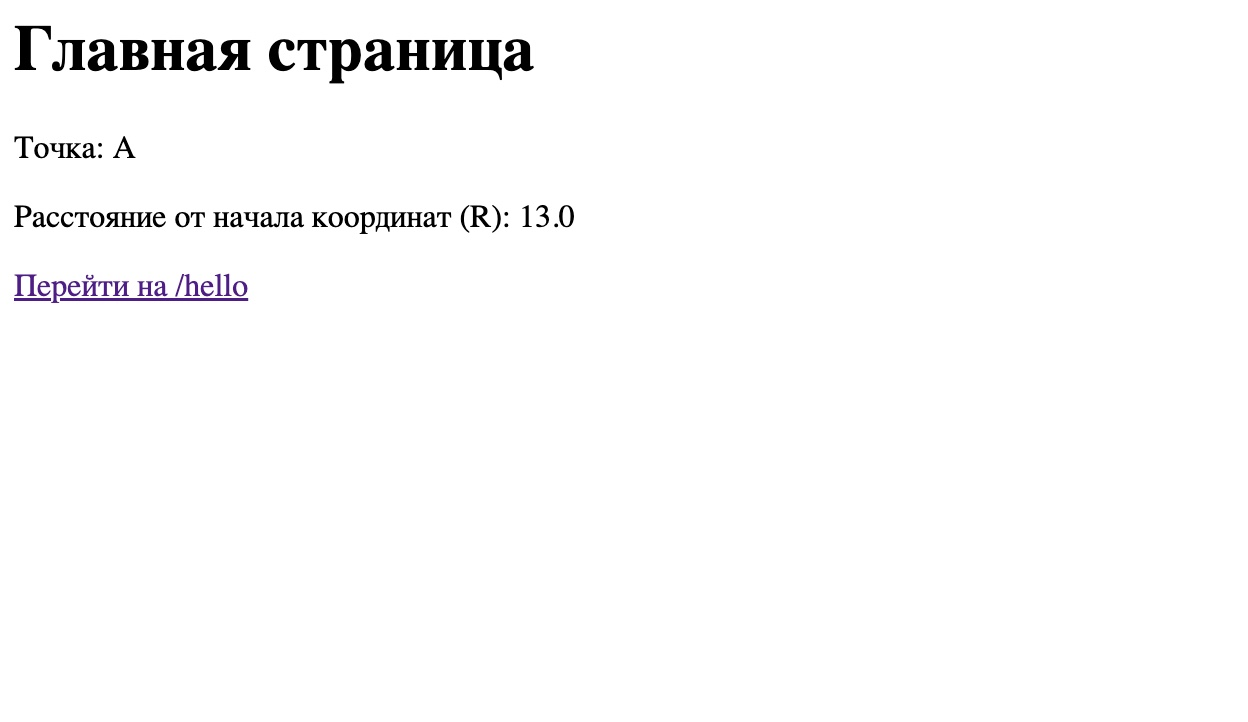
\includegraphics[width=0.8\textwidth]{фото1.jpeg}
    \captionof{figure}{Запуск веб-сервера}

    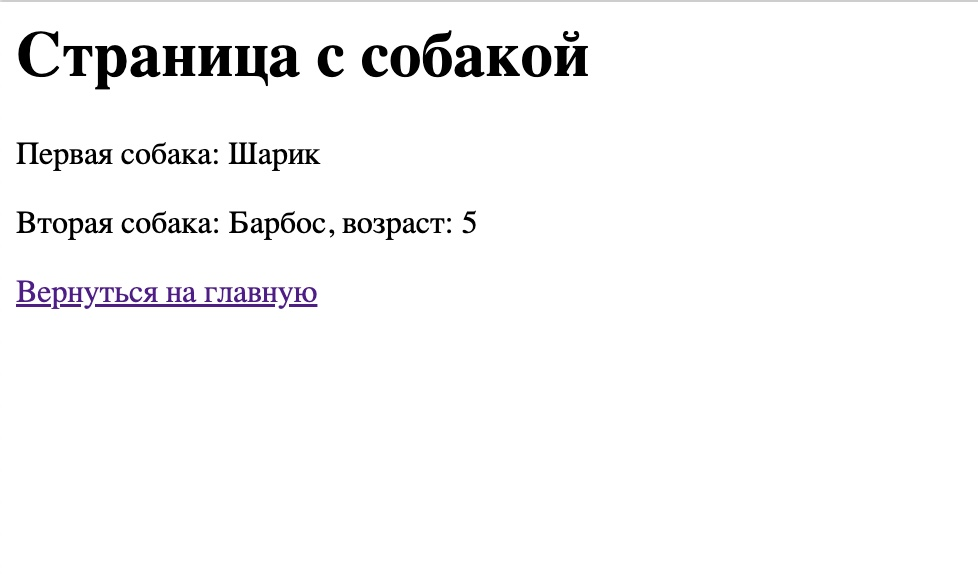
\includegraphics[width=0.8\textwidth]{фото2.jpeg}
    \captionof{figure}{Вложенная страница}
\end{center}
\newpage
\section{Вывод}
В данной лабораторной работе была проведена настройка учетной записи на удаленном VDS-сервере, а также подготовка окружения для компиляции и запуска программ на Java. Был реализован и развернут веб-сервер, который демонстрирует работу программного кода через HTTP-интерфейс. В результате были изучены основы работы с сервером, взаимодействия с клиентами через веб-протокол, а также работа с удаленным сервером в среде Linux.

\end{document}